\documentclass[tikz,border=2pt]{standalone}
\usepackage{tikz}

\begin{document}
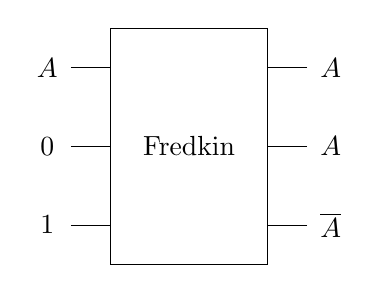
\begin{tikzpicture}[]

\draw (0,0) rectangle (2,3);
\draw (-0.5,0.5) -- (0.0, 0.5);
\node at (-0.8, 0.5) {$1$};
\draw (-0.5,1.5) -- (0.0, 1.5);
\node at (-0.8, 1.5) {$0$};
\draw (-0.5,2.5) -- (0.0, 2.5);
\node at (-0.8, 2.5) {$A$};
\draw (2.5,0.5) -- (2.0, 0.5);
\node at (2.8, 0.5) {$\overline{A}$};
\draw (2.5,1.5) -- (2.0, 1.5);
\node at (2.8, 1.5) {$A$};
\draw (2.5,2.5) -- (2.0, 2.5);
\node at (2.8, 2.5) {$A$};
\node at (1.0, 1.5) {Fredkin};

\end{tikzpicture}
\end{document}
